\documentclass[10pt,a4paper,twoside]{article}
\usepackage{amsfonts}
%\usepackage{ICDD}
\usepackage{graphicx}
\usepackage{booktabs}
\usepackage{amsmath}
\usepackage[hidelinks]{hyperref}
\usepackage{makecell}

\makeatletter
    \def\thebibliography#1{\section*{References\@mkboth
      {REFERENCES}{REFERENCES}}\list
      {[\arabic{enumi}]}{\settowidth\labelwidth{[#1]}\leftmargin\labelwidth
    \advance\leftmargin\labelsep
    \usecounter{enumi}}
    \def\newblock{\hskip .11em plus .33em minus .07em}
    \sloppy\clubpenalty4000\widowpenalty4000
    \sfcode`\.=1000\relax}
    \makeatother

%\addtolength{\oddsidemargin}{1.3cm}
%\addtolength{\evensidemargin}{-0.1cm}
\setlength{\topmargin}{-0.2cm}
%\setlength{\textheight}{20cm} \setlength{\textwidth}{13cm}
\setlength{\textheight}{8.890in} \setlength{\textwidth}{6.3in}
\setlength{\oddsidemargin}{.077in}
\setlength{\evensidemargin}{.077in} \thispagestyle{empty}


\begin{document}
%\tableofcontents
\pagestyle{empty}

\def\SHORTTITLE  {Assessing Visual Tracking in Children with Special Needs: A Tool for Ergotherapists}%

\vspace*{3cm}
%\antet
\markboth{\hfill Gokul Perumbayil Vijayarkrishnan, Anagha Manikathuparambil Baby, Blesson Manjakunnel}{\hfill
\SHORTTITLE}

\begin{center}
{\Large \bf Assessing Visual Tracking in Children with Special Needs: A Tool for Ergotherapists}
\par\vspace*{0.5cm}
{\bf Gokul Perumbayil Vijayakrishnan, Anagha Manikathuparambil Baby, Blesson Manjakunnel }
\end{center}

\vspace*{0.3cm}
%%%%%%%%%%%%%%%%%%%%%%%%%%
%%%%%% PROOF.TEX %%%%%%%%%
%%%%%%%%%%%%%%%%%%%%%%%%%%
\tolerance 10000
\newtheorem{theorem}{Teorem\check{a}}
\newtheorem{lemma}{Lema}
\newtheorem{definition}{Definitie}
\newtheorem{example}{Exemplu}
\newtheorem{xca}{Exercitiu}
\newtheorem{remark}{Observatie}
\newtheorem{proposition}{Propozitie}
\newtheorem{corollary}{Corolar}

%Please use these definitions for Latex entities (theorem, lemma, etc.)
%If you need other definitions add to this list and notify us, by e-mail, about this.
%--------------------------------------

\begin{abstract}

Assessing visual tracking ability in children with special needs is challenging due to the limitations of traditional observational methods, which are often time-consuming, costly, and imprecise, while also struggling to maintain the engagement of the child. Additionally, these methods can be difficult for therapists to interpret. This study proposes a cost-effective eye-tracking tool that enables therapists to evaluate and enhance visual tracking abilities without the need for specialised hardware.

The tool integrates an interactive game to sustain engagement while using a standard webcam to capture gaze data. A deep learning model then processes this data, mapping gaze direction to screen coordinates to generate an interpretable representation of visual tracking performance. Our analysis quantifies the correlation between predicted gaze points and the actual trajectory of a moving object along the x and y axes, providing therapists with a visual representation of gaze behaviour.

By enabling remote assessments and minimizing logistical barriers, this tool enhances accessibility, precision, and efficiency in therapeutic evaluations. It provides an affordable, open-source alternative to conventional eye-tracking systems, usable on any standard computer with a webcam, and supports data-driven intervention strategies to enhance therapeutic outcomes.

\end{abstract}

\section{Introduction}
\label{Intro}

Therapists who work with children with special needs generally rely on observational techniques to assess and address developmental challenges related to communication, attention, and motor skills \cite{Powers2025}. However, such traditional assessment methods are inherently time-consuming, subjective, and constrained in their ability to capture the complex dynamics of a child’s behaviour and participation over time. Furthermore, the requirement for in-person evaluations in specialised facilities poses significant logistical and financial challenges for families, particularly those in geographically remote or resource-limited areas \cite{ramezani2025bench}. These limitations highlight the need for innovative tools that improve the precision and efficiency of therapeutic evaluations while enabling remote accessibility.

Eye tracking technology has emerged as a promising non-invasive approach to assessing gaze patterns and visual attention, offering objective insights into cognitive and motor functions \cite{wolf2021contribution}. Despite its potential to improve therapeutic practices, adoption of such technology in clinical and therapeutic settings remains limited due to the high cost, technical complexity, and dependence on high-precision specialised equipment \cite{CyntiaLimaFonsecaRodrigues2024}. These barriers disproportionately affect underfunded therapy centres and families in rural regions \cite{Hunt2025}, increasing inequalities in access to effective interventions.

This research seeks to address these challenges by developing a cost-effective therapist-focused eye-tracking application designed to provide meaningful, actionable insights into children’s eye movements during therapy sessions. Unlike traditional systems, the proposed tool eliminates the need for expensive high-precision hardware and facilitates remote access through a server-based platform. This approach allows therapists to monitor children’s eye movement data during interactive, game-like activities conducted in home environments. The platform processes and analyses this data, enabling therapists to design personalised intervention strategies without requiring in-person evaluations.

\section{Related Work}
\label{RW}

Eye tracking has been a subject of research interest for many years, with commercial eye trackers available on the market. As of 2020, the most accurate stationary eye-tracking device was the SMI Red, offering an accuracy of 0.4$^{\circ}$ at a cost of approximately \$40,000 \cite{rakhmatulin2020}. However, there remains a need for an affordable, budget-friendly eye-tracking solution, which this study aims to address.

The model-based approach \cite{Wang2015} involves the use of mathematical or computational models to interpret eye movement data. A model-based eye tracking approach \cite{Varghese2023} was used to monitor gaze and provide information to the therapists. Despite its innovative intent, this method had several limitations, including the need for users to maintain a fixed distance from the screen, which restricted flexibility, its ineffectiveness for children who wore glasses, and the generation of insights that lacked significant value. Our approach aims to address these challenges, enhancing both the system's utility and inclusivity.

In contrast, appearance-based models focus on extracting visual features from static images or individual frames to analyse, predict, and interpret patterns \cite{1182180}. Compared to model-based approaches and traditional appearance-based methods, deep learning appearance-based methods demonstrate greater robustness in unconstrained environments, effectively handling extreme head-pose variations, diverse illumination conditions, and occlusions of the eyes and face \cite{Pathirana2022}. This study uses an appearance-based model to estimate the eye gaze.

Eye-tracking technology is a valuable tool for assessing cognitive and social processing in children with special needs, including autism spectrum disorders (ASD), attention deficit hyperactivity disorder (ADHD), and learning disabilities. A recent meta-analysis of 20 eye-tracking studies on face processing in children with ASD found significantly reduced gaze fixation on the eye region, suggesting it as a potential biomarker for ASD \cite{Papagiannopoulou2014}. The study highlights the importance of gaze behaviour in ASD diagnosis and reinforces the need for further research to enhance eye-tracking applications in special education and therapy.

\section{Methodology}
\label{M}

The study adopts a quantitative framework to design, implement, and validate a novel tool to assist ergo therapists in precisely analysing eye movements in children with special needs. The primary goal is to assess participants' visual tracking capabilities through an interactive game, leveraging cutting-edge deep learning techniques and geometric transformations to deliver actionable insights. A camera calibrated using the chequerboard method will be provided to the user for operating this tool; alternatively, users can perform the camera calibration with the chequerboard themselves at their convenience before using the tool. The study is structured into three comprehensive phases: data acquisition through a custom-designed game, gaze estimation and screen coordinate mapping, and performance evaluation and therapeutic insight generation. Figure \ref{fig:flowchart} shows the overall architecture of the software.

\begin{figure*}[htbp]
    \centering
    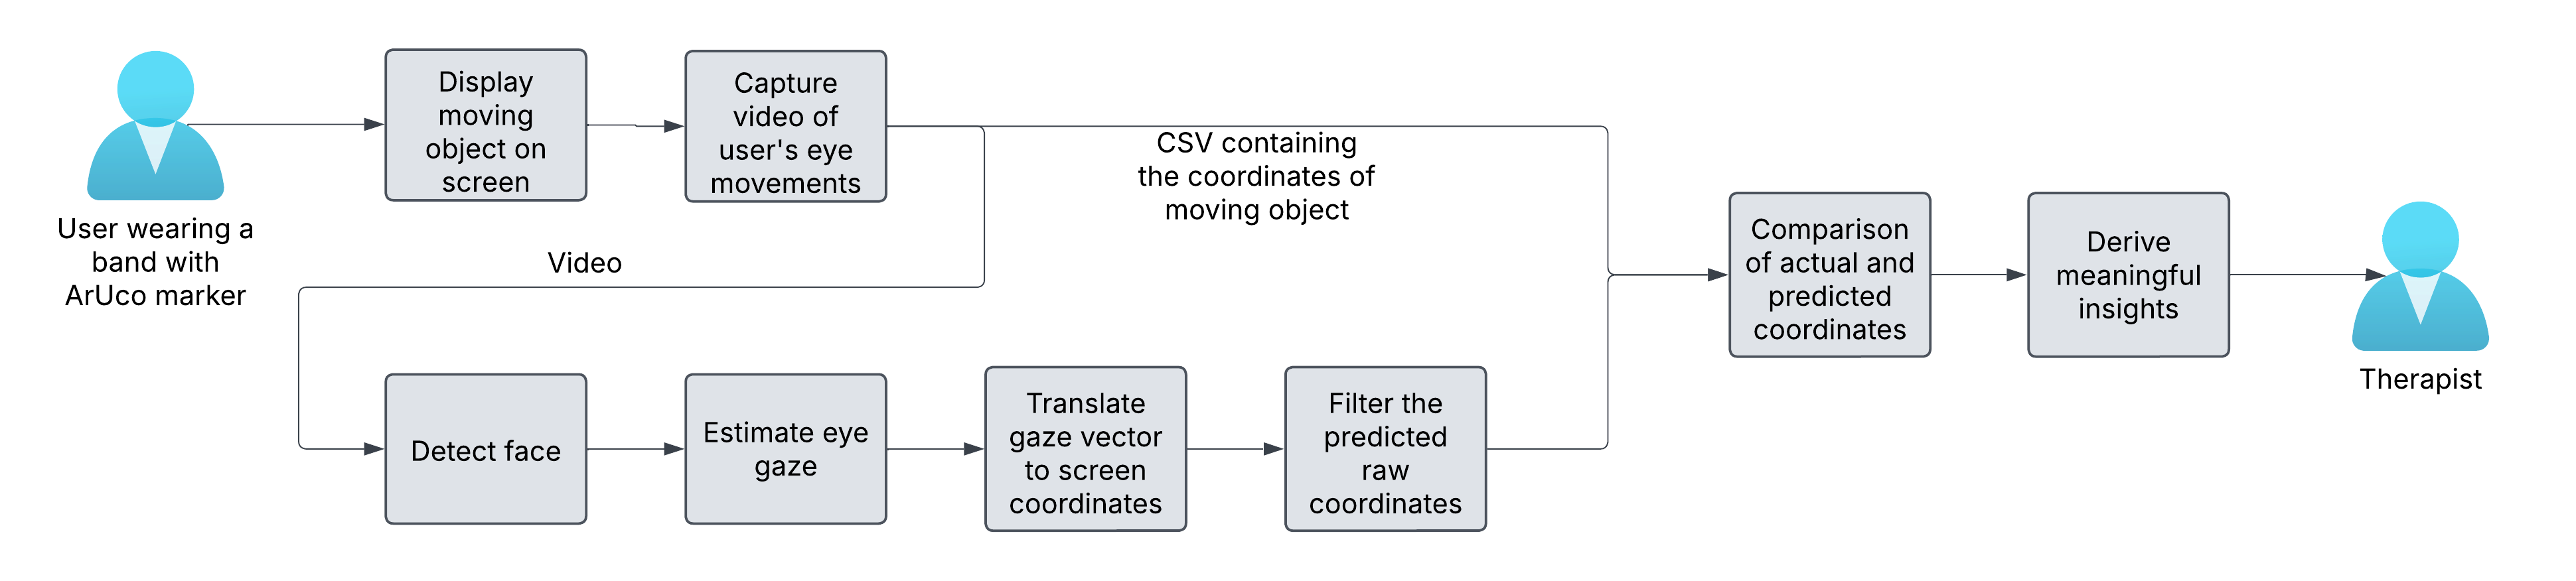
\includegraphics[width=\textwidth]{image/flowchart.png}
    \caption{The diagram illustrates the system architecture for gaze tracking and analysis. The process begins with a user wearing a band with an ArUco marker. The recorded video is processed to detect the face, estimate eye gaze, and translate gaze vectors into screen coordinates. A filtering step refines the predicted raw coordinates before they are compared with actual object coordinates. The final insights, derived from this comparison, assist a therapist in understanding gaze behaviour.}
    \label{fig:flowchart}
\end{figure*}

\subsection{Data Acquisition via Interactive Game}
\label{data}

The data acquisition phase is central to ensuring the accuracy and relevance of subsequent analysis. A custom-designed game engages participants while systematically capturing their gaze behaviour. The game features a visually appealing cartoon character that moves across the screen along predefined trajectories: horizontal, vertical, and diagonal. These simple trajectories focus on baseline gaze-tracking metrics and coordination, without imposing undue cognitive load on the participants. During the game, the speed of the character is adjustable, and the interface is designed to maintain the attention and interest of children, thereby ensuring high-quality data capture.

The trajectories are logged in real time, and the precise screen coordinates of the moving character are recorded at each frame in a CSV file for later analysis. This structured data serves as a reference for evaluating gaze alignment. Although more intricate motion patterns, such as circular or zigzag trajectories, could provide deeper insights into complex gaze-tracking behaviours, they are deliberately excluded in this initial phase to minimize complexity and enhance the robustness of the foundational metrics.

Participants are seated approximately 60 cm from the screen, ensuring a consistent spatial geometry between the camera, monitor, and gaze direction. A standard webcam records video footage of the participant’s face during the game, capturing fine-grained frame-by-frame details of their eye movements. To account for participants’ positioning relative to the screen, each participant wears a headband equipped with an ArUco marker \cite{GARRIDOJURADO20142280}, a computer vision tool that facilitates accurate real-time distance measurement. This ensures the tool remains cost-effective by eliminating the need for expensive, specialised hardware to measure the user's distance from the screen, a critical factor affecting the conversion of gaze coordinates into screen coordinates. Figure \ref{fig:game} illustrates the game interface alongside the participant actively tracking the moving object.

\begin{figure*}[htbp]
    \centering
    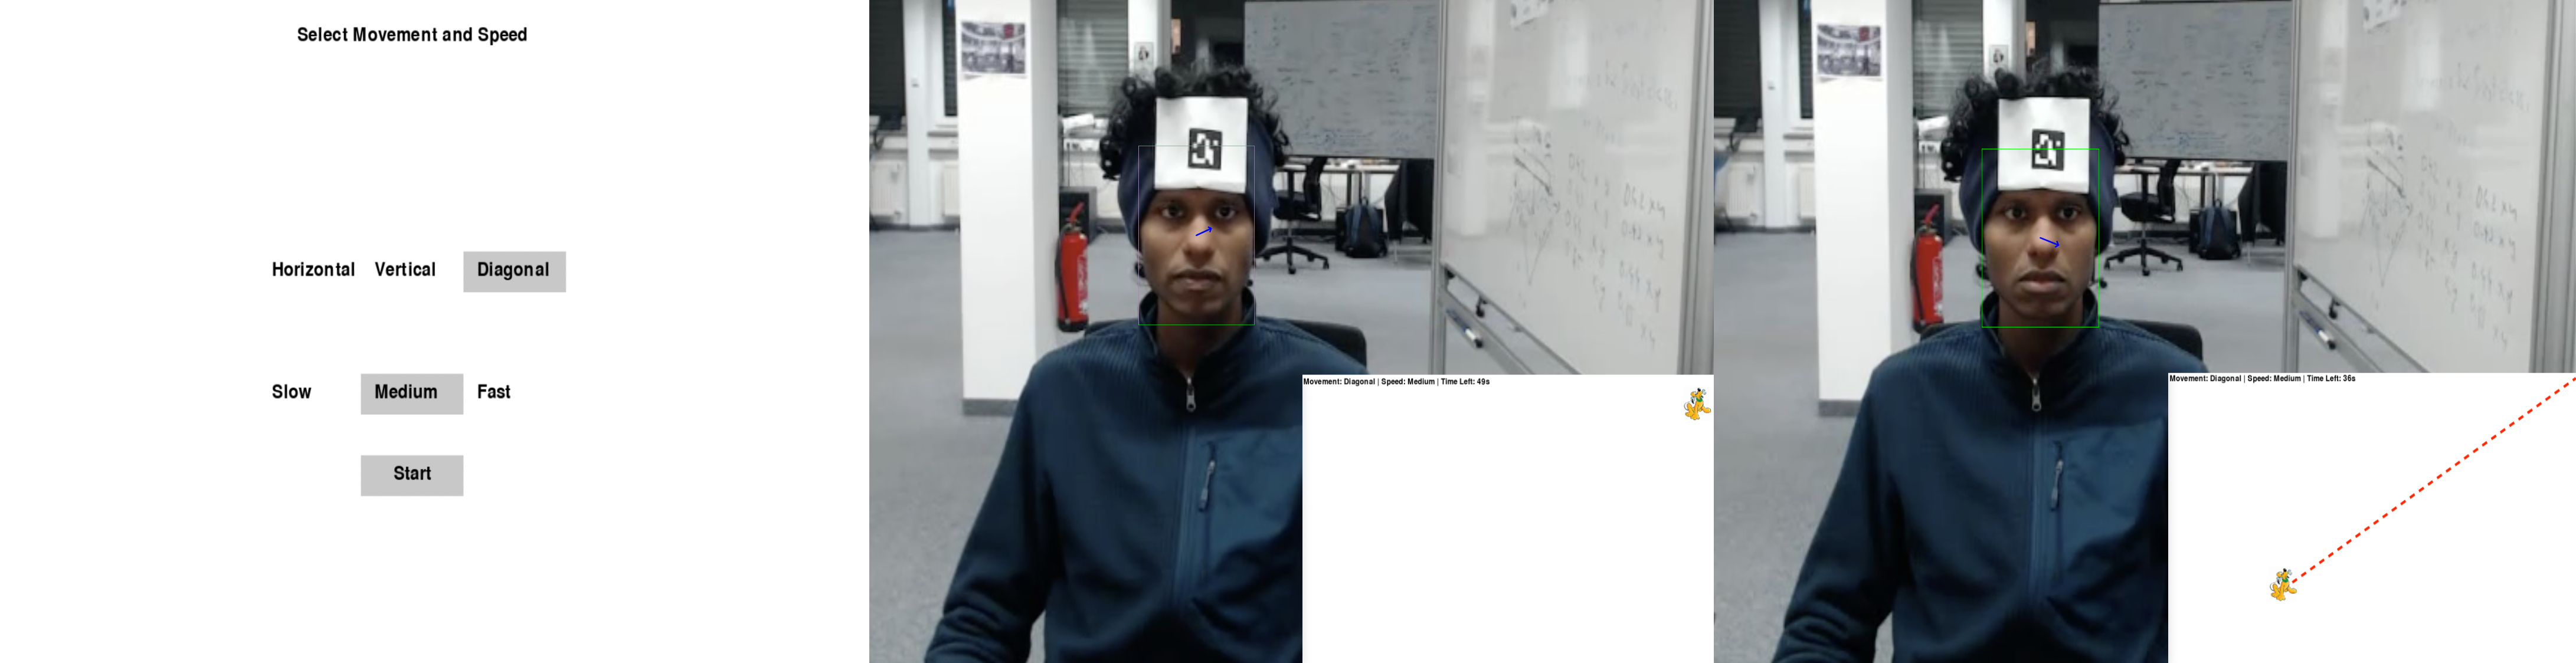
\includegraphics[width=\textwidth]{image/game_ui.png}
    \caption{A person wearing a headband with an ArUco marker is trying to track the movement of a cartoon character in a particular direction (in this case, diagonal movement).}
    \label{fig:game}
\end{figure*}

\subsection{Gaze Estimation and Mapping to Screen Coordinates}
\label{gaze}

In the second phase, the captured video frames undergo processing using L2CS-Net \cite{abdelrahman2022}, a pre-trained deep learning model specifically designed for gaze estimation and trained on the Gaze360 dataset \cite{kellnhofer2019}. L2CS-Net predicts yaw and pitch angles, which correspond to gaze direction's horizontal and vertical components, respectively. This model is selected for its demonstrated superiority over traditional approaches such as regression-based methods or geometric models \cite{abdelrahman2022}. While conventional techniques often require controlled environments and manual feature engineering, L2CS-Net’s reliance on large-scale datasets allows it to generalize effectively across diverse settings, making it highly robust and adaptive.

One critical challenge addressed during this phase is the variability in participants' distance from the screen. The ArUco marker enables the computation of the participant's distance from the screen for each video frame, which is subsequently utilised in further calculations. The distance $d$ of the participant from the screen can be calculated using the magnification formula for a lens as

\begin{equation}
\label{eq1}
    d = \frac{f \cdot h_o}{h_i}
\end{equation}

where $f$ is the focal length of the camera obtained using camera calibration, $h_o$ is the actual width of the ArUco marker in cm and $h_i$ is the width of the ArUco marker in pixels. Once the distance $d$ is calculated, a geometric transformation is applied to map the gaze angles (yaw and pitch) to precise screen coordinates, effectively accounting for the position of the participant relative to screen, as shown in figure \ref{fig:translation}. The equations for converting gaze angles (yaw and pitch) to pixel coordinates on the screen are given by:

\begin{equation}
\begin{array}{ll}
    x = -d \cdot \tan(\text{yaw}), & \quad
    y = -d \cdot \arccos(\text{yaw}) \cdot \tan(\text{pitch})
\end{array}
\label{eq2}
\end{equation}

where \( d \) is the screen distance in cm, \( \text{yaw} \) and \( \text{pitch} \) are angular values in radians. The additional term $\arccos(\text{yaw})$ in equation (\ref{eq2}) is an empirical scaling factor to adjust vertical displacement based on horizontal deviation. The conversion from cm to pixel coordinates with top left as origin is as follows:

\begin{equation}
\begin{array}{ll}
    x_{\text{pixel}} = \left( \dfrac{x + \frac{W_{\text{cm}}}{2}}{W_{\text{cm}}} \right) \times W_{\text{pixels}}, & \quad
    y_{\text{pixel}} = \left( \dfrac{y + \frac{H_{\text{cm}}}{2}}{H_{\text{cm}}} \right) \times H_{\text{pixels}}
\end{array}
\label{eq3}
\end{equation}

where \( W_{\text{cm}} \) and \( H_{\text{cm}} \) are the width and height of the screen in cm, and \( W_{\text{pixels}} \) and \( H_{\text{pixels}} \) are the screen width and height in pixels.

\begin{figure} [h!]
    \centering
    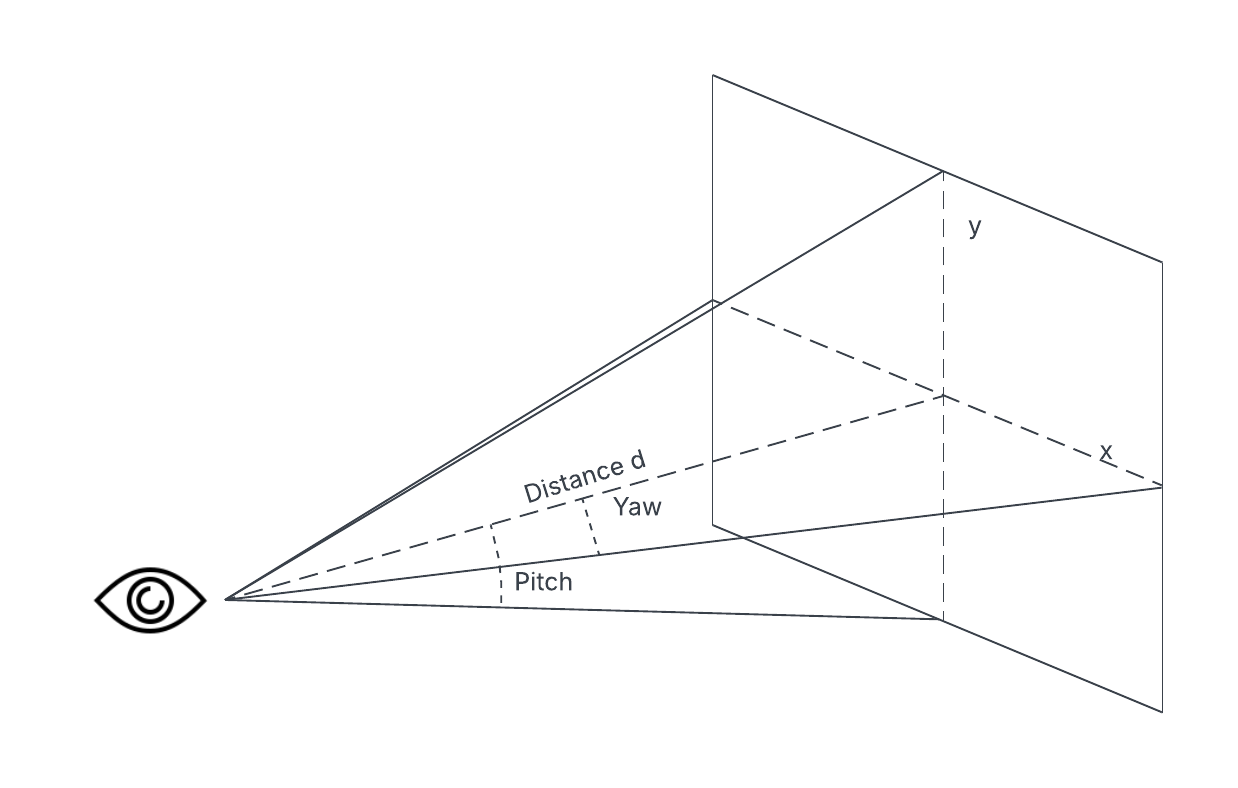
\includegraphics[width=0.6\linewidth]{image/screen_translation.png}
    \caption{Translation of yaw and pitch angles into screen coordinates (x and y).}
    \label{fig:translation}
\end{figure}

Since the raw screen coordinates obtained from gaze tracking are often noisy due to head movements, eye blinks, and lighting variations, a Kalman filter \cite{kalman1960new} is applied to smooth the data and handle missing values. By recursively estimating the true gaze position based on both past predictions and the current noisy measurements, the filter improves tracking accuracy. A constant velocity motion model is assumed, as the video is recorded at 30 FPS. The state vector of the Kalman filter consists of four components:

\begin{equation}
\label{eq4}
\mathbf{x} = \begin{bmatrix} x \\ y \\ v_x \\ v_y \end{bmatrix}
\end{equation}

where \( x \) and \( y \) represent the estimated gaze position on the screen (after filtering), while \( v_x \) and \( v_y \) represent the estimated gaze velocity in the horizontal and vertical directions, respectively. The system follows a linear motion model:

\begin{equation}
\label{eq5}
\mathbf{x}_k = \mathbf{F} \mathbf{x}_{k-1} + \mathbf{w}_k
\end{equation}

where \( \mathbf{F} \) is the state transition matrix defined as:

\begin{equation}
\label{eq6}
\mathbf{F} =
\begin{bmatrix}
1 & 0 & \Delta t & 0 \\
0 & 1 & 0 & \Delta t \\
0 & 0 & 1 & 0 \\
0 & 0 & 0 & 1
\end{bmatrix}
\end{equation}

with \( \Delta t = \frac{1}{\text{FPS}} \;\text{s} \), with FPS denoting the number of frames per second. The process noise \( \mathbf{w}_k \) accounts for small random variations in motion. The Kalman filter updates its estimates using the measurement model, which includes only two components, \( x \) and \( y \), corresponding to the observed gaze positions from equation (\ref{eq3}).

\begin{equation}
\label{eq7}
\mathbf{z}_k = \mathbf{H} \mathbf{x}_k + \mathbf{v}_k
\end{equation}

where \( \mathbf{v}_k \) represents measurement noise, and \( \mathbf{H} \) is the observation matrix given by equation (\ref{eq8}).

\begin{equation}
\label{eq8}
\mathbf{H} =
\begin{bmatrix}
1 & 0 & 0 & 0 \\
0 & 1 & 0 & 0
\end{bmatrix}
\end{equation}

At each time step, the filter predicts the next gaze position based on the current state estimate and corrects it using the incoming measurements, effectively reducing noise and ensuring smoother tracking.

\subsection{Performance Evaluation and Metrics Extraction}
\label{perf}

The final phase involves a rigorous comparison of the mapped gaze coordinates with the recorded coordinates of the moving cartoon character. This comparison yields quantitative metrics that offer insights into the participant’s visual tracking capabilities. The key metrics include:

\begin{itemize}
    \item Cross correlation: Measures how well the gaze trajectory follows the object movement over time. A high correlation (closer to 1) means the gaze movement aligns well with the object movement. Cross-correlation has been widely used in gaze tracking research to quantify alignment \cite{Duchowski2007}.

    \begin{equation}
    \label{cross}
        \rho_{x} =
        \frac{\sum_{i=1}^{N} (x_{\text{g}, i} - \bar{x}_{\text{g}}) (x_{\text{obj}, i} - \bar{x}_{\text{obj}})}
        {\sqrt{\sum_{i=1}^{N} (x_{\text{g}, i} - \bar{x}_{\text{g}})^2 \sum_{i=1}^{N} (x_{\text{obj}, i} - \bar{x}_{\text{obj}})^2}}
    \end{equation}


    where \( x_{\text{g}, i} \) represents the gaze position at time \( i \), and \( \bar{x}_{\text{g}} \) denotes the mean gaze position. Similarly, \( x_{\text{obj}, i} \) represents the object position at time \( i \), while \( \bar{x}_{\text{obj}} \) refers to the mean object position.

    \item Gaze Jitter: Measures how much the gaze position fluctuates within short time intervals. High jitter (closer to 1) indicates noisy tracking, while low jitter suggests stable gaze tracking. This metric has been used to assess gaze stability and visual attention in experimental psychology \cite{Engbert2003}.

    \begin{equation}
    \label{jitter}
        \text{Jitter} =
        \frac{1}{N} \sum_{i=1}^{N}
        \left( (x_{\text{g}, i} - x_{\text{g}, i-1})^2 + (y_{\text{g}, i} - y_{\text{g}, i-1})^2 \right)
    \end{equation}

    where \( x_{\text{g}, i} \) and \( y_{\text{g}, i} \) represent the gaze coordinates at time \( i \), while \( x_{\text{g}, i-1} \) and \( y_{\text{g}, i-1} \) denote the gaze coordinates at time \( i-1 \). Additionally, \( N \) represents the total number of gaze samples.
\end{itemize}

These metrics collectively provide a comprehensive assessment of visual tracking performance, helping to identify specific visual-motor challenges. A low correlation in certain axes (e.g., horizontal vs. vertical) may indicate difficulties in gaze coordination or tracking consistency. Such insights enable ergo-therapists to design personalised interventions. For instance, if a child demonstrates strong horizontal tracking but weaker vertical tracking, targeted exercises can be introduced to improve vertical gaze control, ultimately enhancing overall tracking ability and engagement in daily activities.

The proposed approach prioritizes cost-effectiveness without compromising performance. By utilizing a standard webcam and open-source software tools, the methodology avoids the prohibitive costs associated with specialised eye-tracking hardware, such as Tobii \cite{tobii_reference} or Pupil Labs systems \cite{pupil_reference}. The proposed tool enables children to complete the test at home without requiring visits to a testing centre, while therapists can remotely access insights and provide personalised recommendations. The software-driven nature of this tool achieves an optimal balance between precision, affordability, and ease of implementation.

\section{Experiments and evaluation}
\label{Exp}

\subsection{Evaluation Framework}
\label{eval}

To ensure the reliability and generalization of the proposed eye-tracking tool, a Python-based evaluation framework has been developed. This framework systematically analyses the gaze data collected during the interactive game by comparing participants’ gaze behaviour with the predefined trajectories of the moving character. A robust baseline for gaze behaviour in individuals with normal vision is established using mean and standard deviation. This baseline serves as a critical reference point for future comparative studies using Z-score involving children with special needs, recognizing the challenges of directly acquiring data from this population. By adopting a quantitative and systematic approach, the framework validates the ability of the tool to provide actionable information to therapists while ensuring its adaptability across diverse user groups.

\subsection{Experimental Setup}
\label{setup}

To evaluate the performance of the tool under simulated real-world conditions, validation experiments were conducted with seven participants, all of whom had normal vision. Three participants completed the experiment twice to assess repeatability. The evaluation focused on two key metrics: correlation of gaze position along the x and y axes and gaze jitter. All experiments were conducted in a controlled environment to reduce external influences, such as inconsistent lighting or screen glare. Since participants are expected to complete this assessment in a home environment, a well‐lit indoor room was selected for the experimental setup. The participants were placed at a standardised distance (60 cm) from the screen, ensuring uniform spatial alignment between the camera, the monitor, and the participant.

To support these experiments, the system used by the participants consisted of a standard computer equipped with an octa-core processor, 8 GB of RAM, a 1080p webcam capable of recording at 30 frames per second, and a 25-inch Full HD display. The system responsible for video processing and result generation was configured with a more powerful setup, featuring a 32-core CPU, 16 GB or more of RAM, at least 8 GB of GPU memory to handle advanced processing tasks and a minimum of 1 TB of storage. These specifications ensured seamless integration between the two systems, enabling efficient remote monitoring and accurate analysis of gaze data.

\subsection{Results}
\label{result}

Figure~\ref{fig:plot} illustrates the trajectory of the object in the game along with the gaze trajectories of the participants after applying filtering to the raw gaze coordinates. The plot reveals that, during the initial frames, gaze positions deviate significantly from the object's path. This is likely because, at the start of the game, participants anticipate the object's initial position and direction of movement rather than actively tracking it. However, after these initial frames, gaze trajectories align more closely with the object's motion, indicating successful tracking.

\begin{figure*}[h]
    \centering
    \begin{tabular}{ccc}
        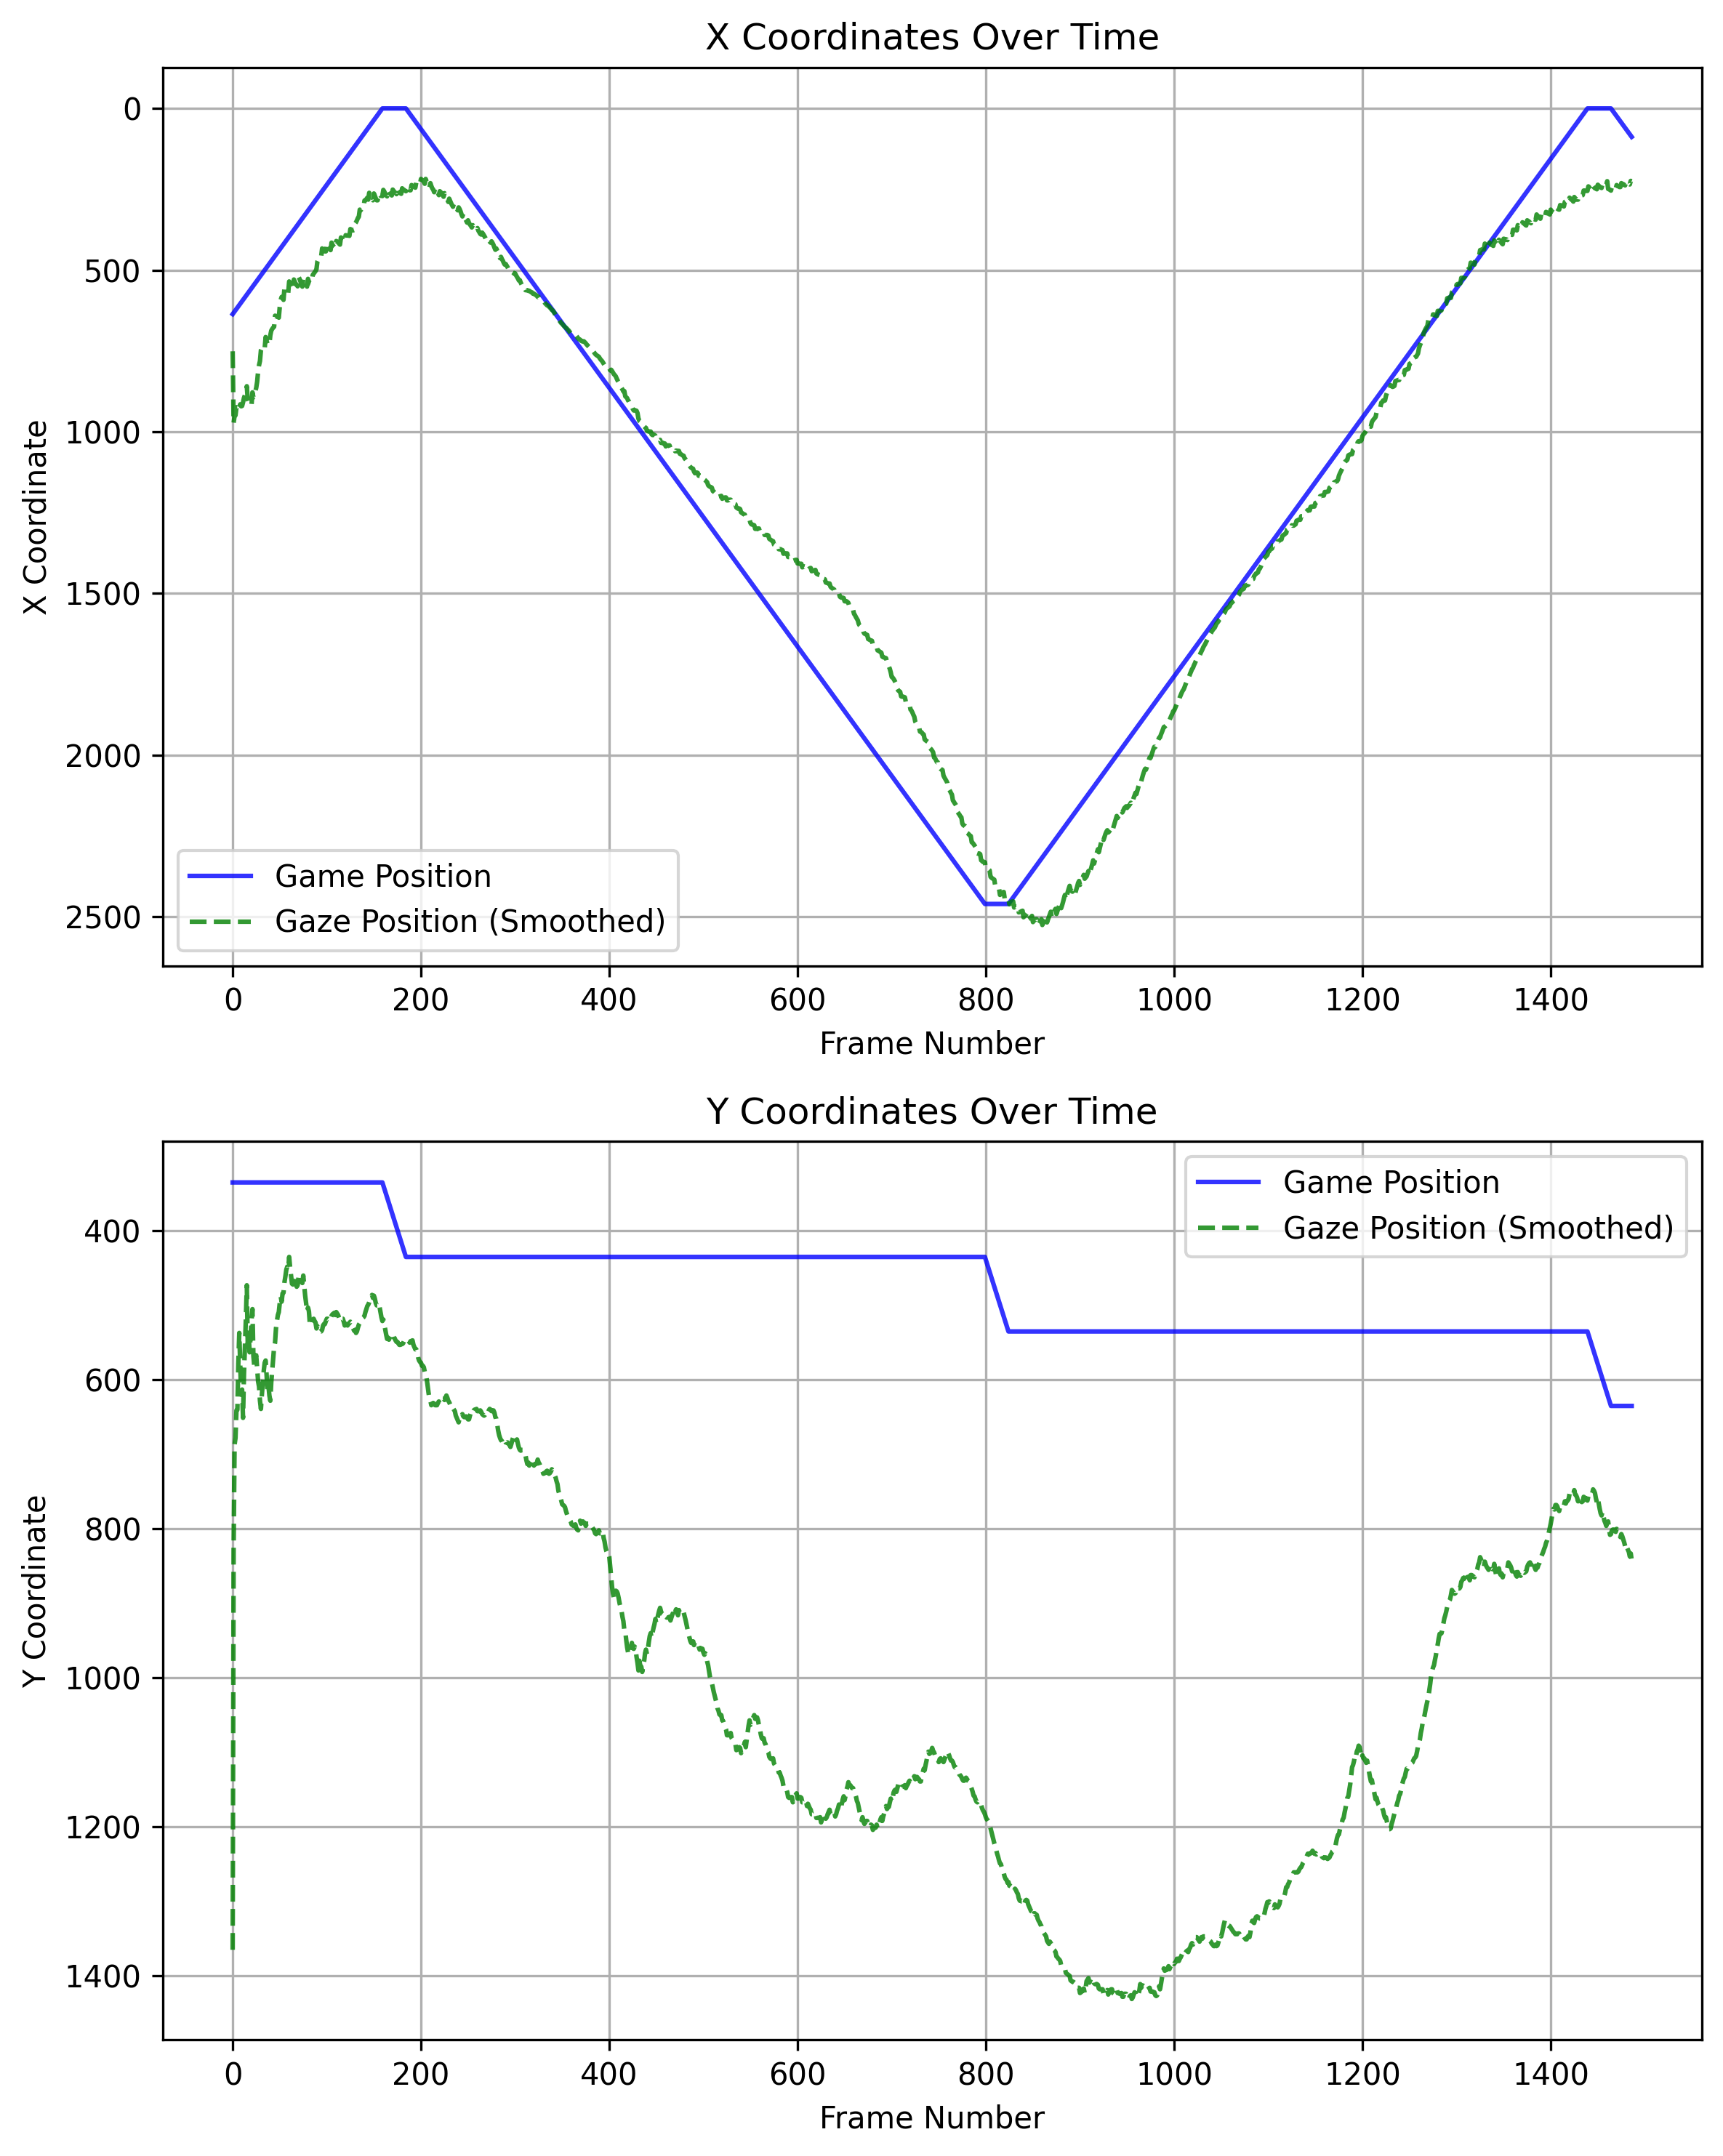
\includegraphics[width=0.3\textwidth]{image/horizontal.png} &
        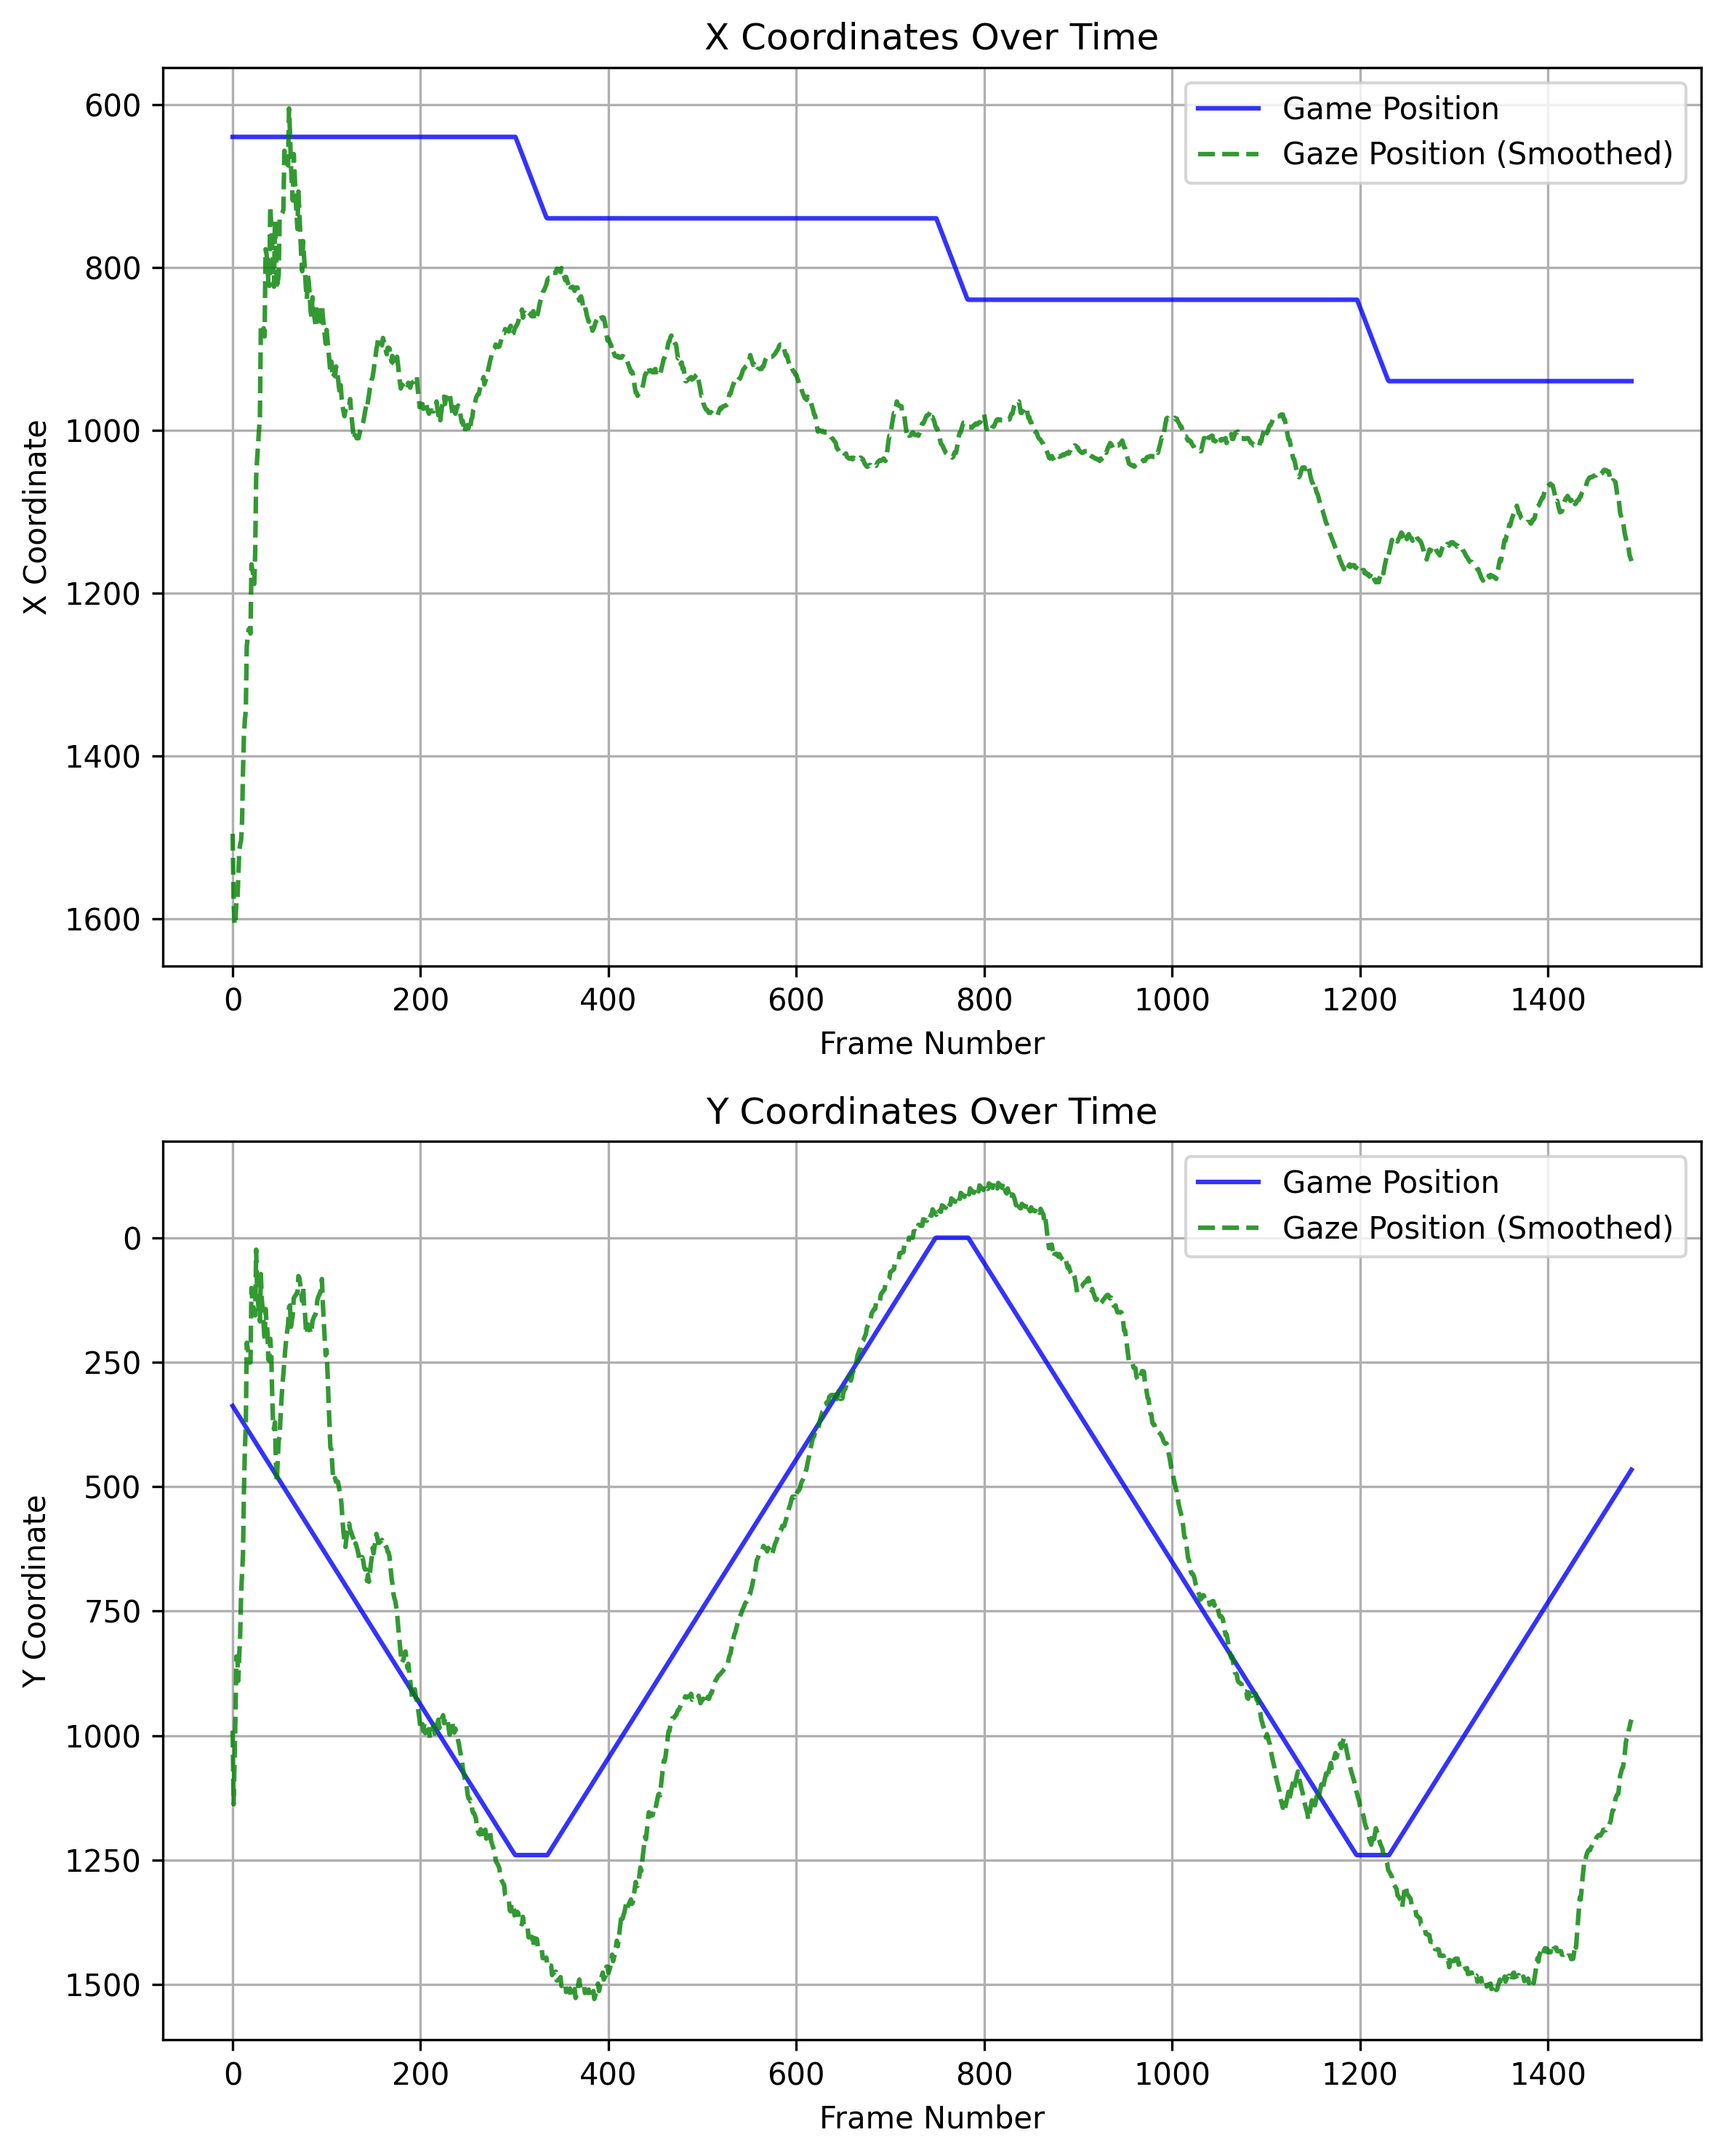
\includegraphics[width=0.3\textwidth]{image/vertical.png} &
        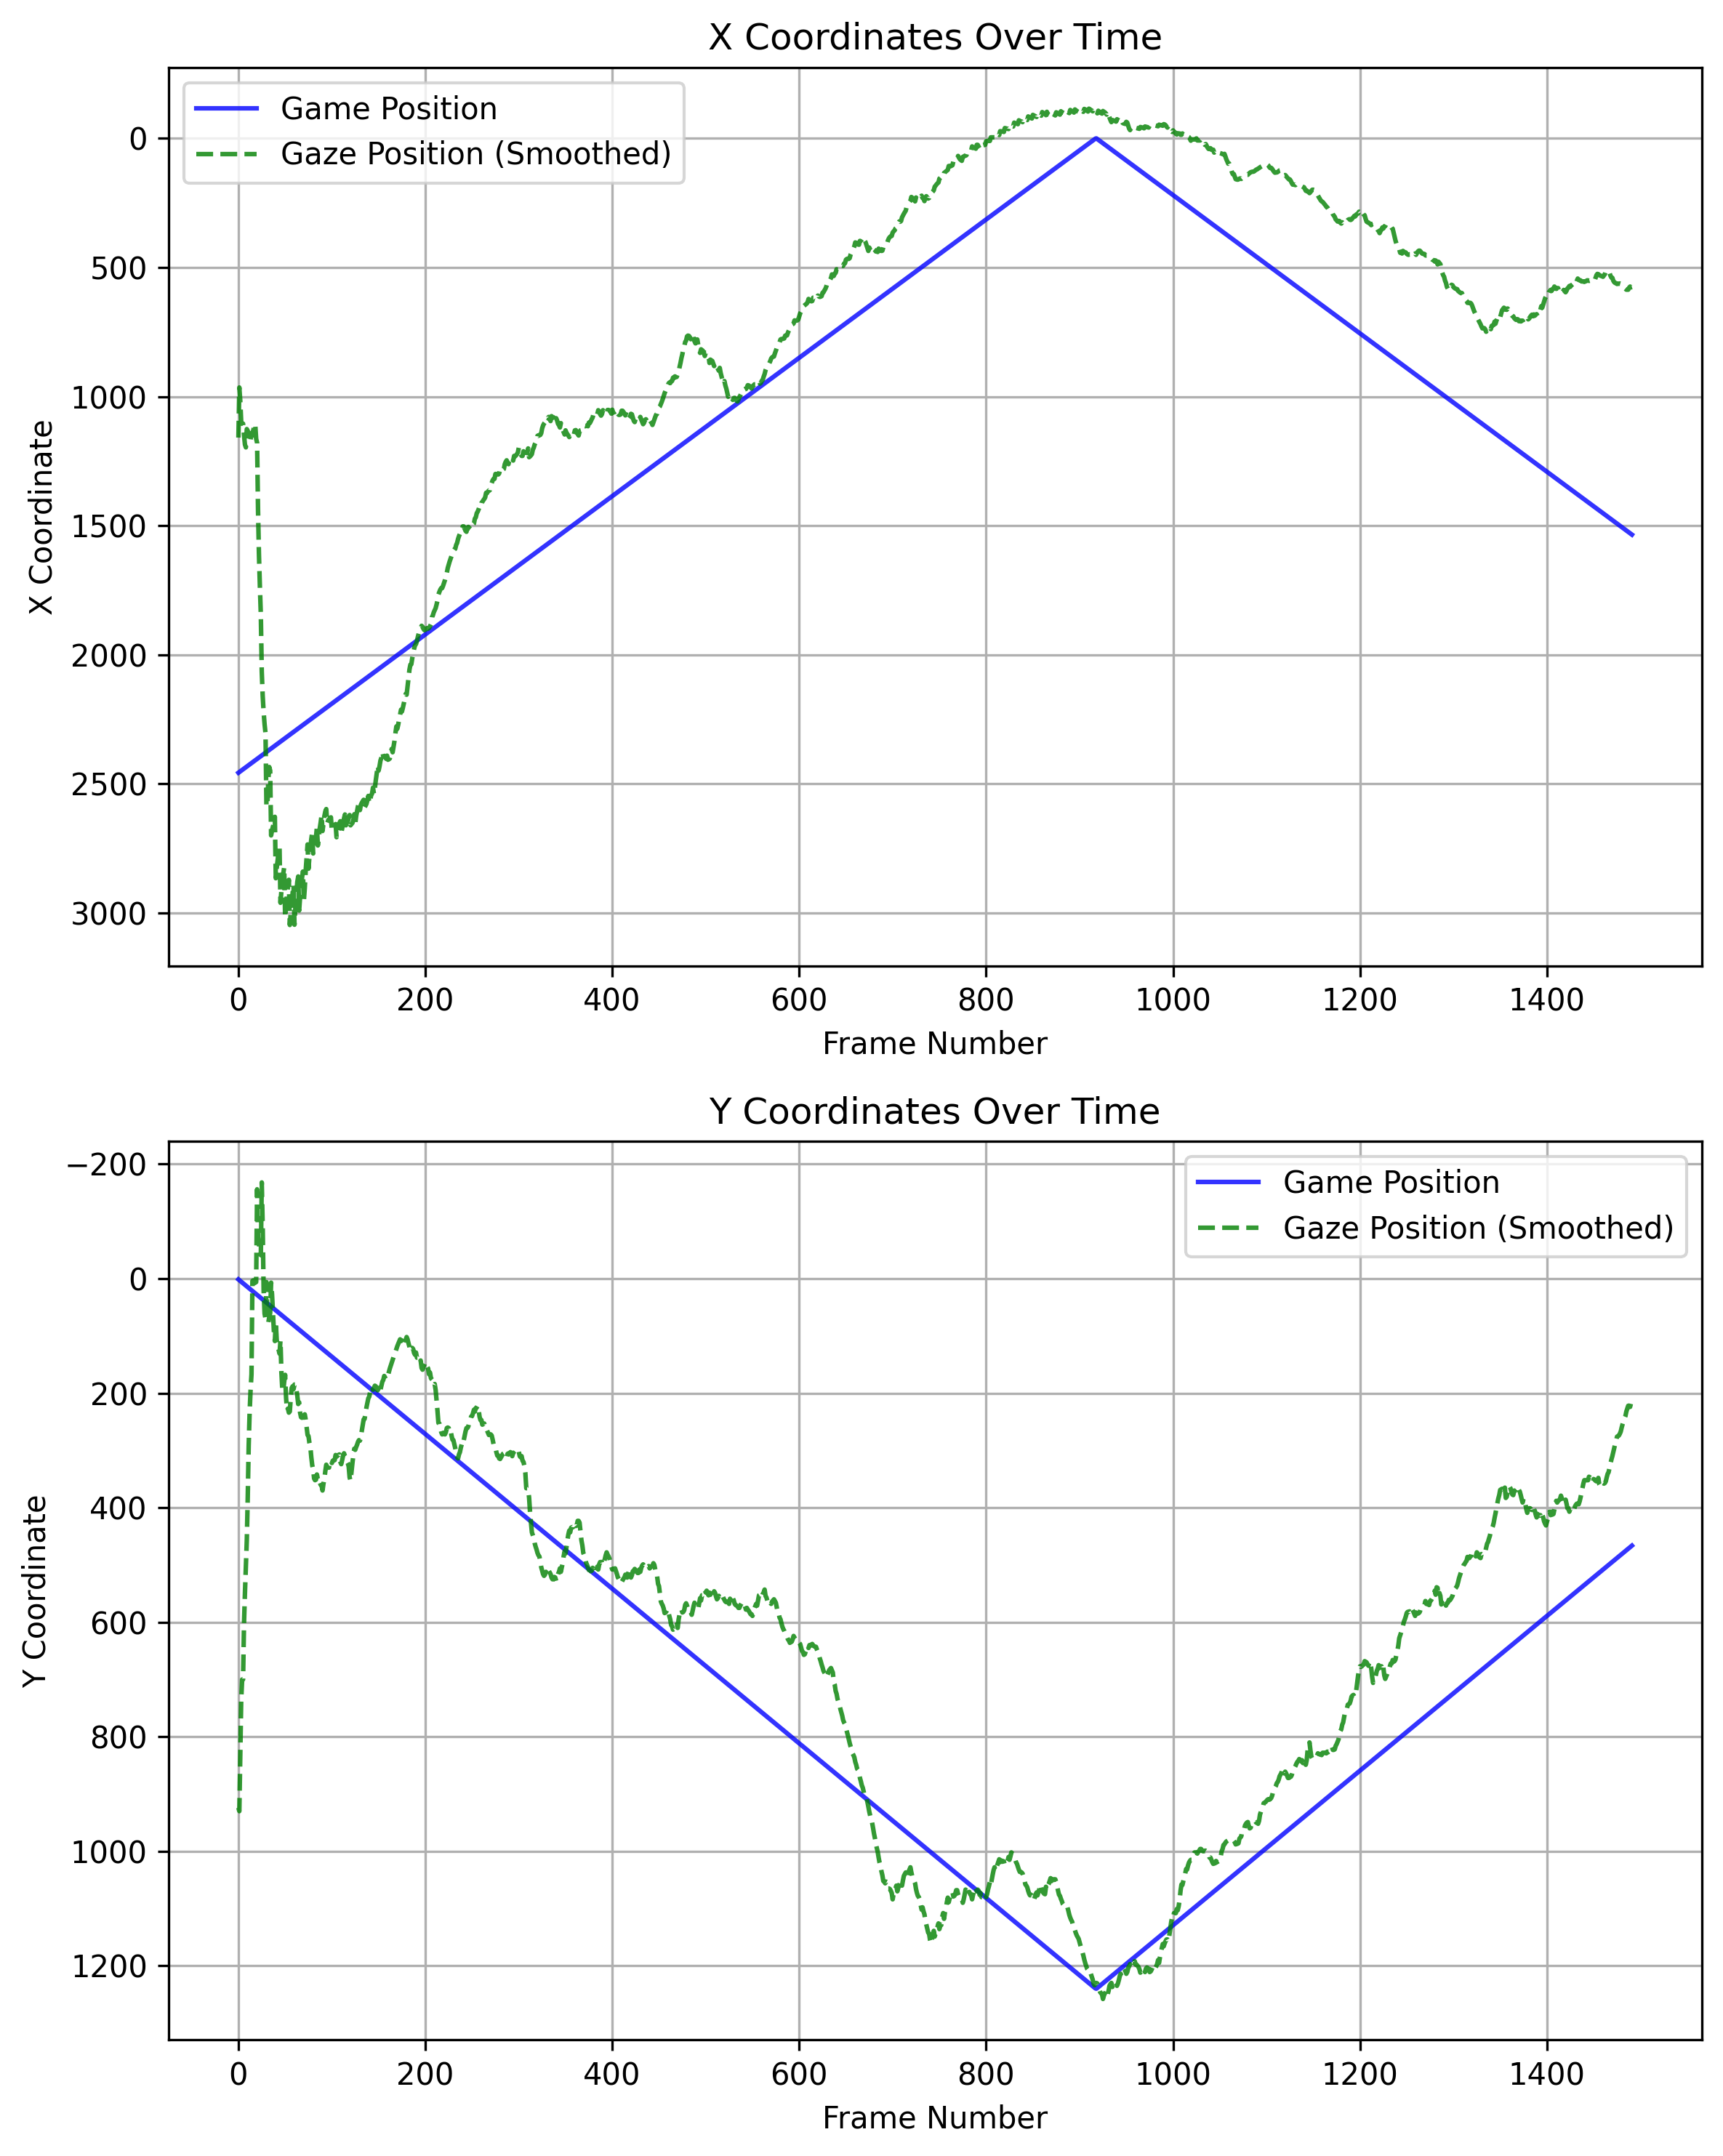
\includegraphics[width=0.3\textwidth]{image/diagonal.png} \\
        (a) Horizontal movement & (b) Vertical movement & (c) Diagonal movement
    \end{tabular}
    \caption{Plots showing the actual movement of an object in the game and the predicted gaze trajectory along the x and y axes. The displayed plots correspond to the best-performing participant for each of the horizontal, vertical, and diagonal movements.}
    \label{fig:plot}
\end{figure*}

Additionally, the results show that for horizontal object movement, tracking accuracy is higher along the x-axis, while deviations occur along the y-axis. Conversely, for vertical object movement, tracking is more accurate along the y-axis, with greater deviations in the x-axis. These deviations may be attributed to slight changes in head orientation or involuntary eye blinks, which are difficult to control.

Table \ref{metr} provides a comprehensive summary of the experimental data. It details the mean values and the associated standard deviations for the correlations along the x and y axes. In addition, the table includes the normalised gaze jitter. The data represent the averages computed from seven participants over ten experimental trials. High correlation values in the x-direction for horizontal object movement and in the y-direction for vertical object movement, along with overall low jitter, suggest that the tracking performance aligns with the expected results for the typical population. The data presented in Table ~\ref{metr} can be used as a baseline for comparison. When the tool is applied to children with special needs, individual performance can be evaluated using Z scores, which indicate how many standard deviations a specific data point is from the population mean. For example, if the mean y-axis correlation ($\mu$) for the diagonal movement is $0.83$ with a standard deviation ($\sigma$) of $0.13$, and a child’s score ($X$) is $-0.37$, the Z-score is computed as,
\begin{equation}
     Z = \frac{X - \mu}{\sigma} = \frac{-0.37 - 0.83}{0.13} = -9.23
\end{equation}

This indicates that the child’s performance is nine standard deviations below the typical mean, suggesting a potential difficulty in horizontal tracking. Such quantifiable comparisons enable tracking of a child’s progress over time, allowing for the refinement of interventions and personalised therapeutic strategies.

\begin{table}[h!]
    \centering
    \begin{tabular}{lccc}
        \toprule
        Metric & Horizontal & Vertical & Diagonal \\
        \midrule
        Correlation X & \textbf{0.97 ± 0.01} & 0.58 ± 0.26 & \textbf{0.94 ± 0.03}\\
        Correlation Y & 0.33 ± 0.46 & \textbf{0.84 ± 0.05} & \textbf{0.83 ± 0.13}\\
        Gaze Jitter & 0.13 ± 0.06 & 0.11 ± 0.08 & 0.21 ± 0.16 \\
        \bottomrule
    \end{tabular}
     \caption{Result statistics — mean and standard deviation of metrics. The table indicates that the x-coordinate correlation is high during horizontal movements. The y-coordinate correlation is notably elevated during vertical movements. Additionally, for diagonal movements, both the x- and y-coordinate correlations are high.}
      \label{metr}
\end{table}

Table \ref{metr1} presents the mean and standard deviation of metrics without the application of the Kalman filter. The comparison between Table \ref{metr} and Table \ref{metr1} indicates that the application of the Kalman filter enhances the correlation values. In Table \ref{metr}, the x-coordinate correlation is higher for horizontal and diagonal movements compared to Table \ref{metr1}. Similarly, the y-coordinate correlation is notably stronger in Table \ref{metr}, especially in vertical and diagonal movements. Table \ref{metr1} shows a higher gaze jitter value and the application of the Kalman filter gives a significant reduction in noise in gaze tracking.

\begin{table}[h!]
    \centering
    \begin{tabular}{lccc}
        \toprule
        Metric & Horizontal & Vertical & Diagonal \\
        \midrule
        Correlation X & \textbf{0.92 ± 0.06} & 0.34 ± 0.20 & \textbf{0.89 ± 0.05}\\
        Correlation Y & 0.27 ± 0.36 & \textbf{0.78 ± 0.10} & \textbf{0.71 ± 0.14}\\
        Gaze Jitter & 16.22 ± 9.96 & 15.28 ± 8.13 & 16.37 ± 8.99 \\
        \bottomrule

    \end{tabular}
     \caption{Result statistics — mean and standard deviation of metrics without using Kalman filter. The comparison with Table \ref{metr} highlights the impact of filtering. }
      \label{metr1}
\end{table}

\section{Conclusion and future work}
\label{conclusion}

This study introduced a cost-effective, deep learning-based eye-tracking tool to assess visual tracking abilities in children with special needs. Given the challenges of directly testing this population, we established a baseline using data from a neurotypical population, demonstrating the accuracy of the tool with minimal jitter. Using a standard webcam and an interactive game, our approach provides an accessible and engaging alternative to traditional observational methods, reducing logistical barriers while enhancing the precision of the evaluation. The structured methodology of the tool, which combines gaze estimation, motion trajectory analysis, and quantitative performance metrics, creates a solid framework for future improvements.

In future work, we intend to integrate head pose estimation to address involuntary head movements, thus further enhancing tracking accuracy. We also plan to incorporate additional gaze metrics—such as latency, fixation sequences, and gaze heatmaps—to provide more comprehensive insights into visual tracking behaviours and improve the overall interpretability of results.

We intend to increase the pool of participants beyond the 7 individuals involved in this study, with the aim of approximately 30 to 40 participants to establish a more robust baseline and increase the validity of our findings. Since children with normal vision and children with special needs are our primary focus, we intend to include them in the participant pool. In addition, further refinements to the interactive game design will enhance participant engagement, yielding higher‐quality data and more accurate tracking. We also plan to develop dedicated user profiles for children, therapists, and parents, allowing for more tailored assessments and supporting long‐term progress monitoring.

Finally, we plan to extend the tool’s applicability to other therapeutic contexts such as cognitive rehabilitation and neurological assessments broadening its impact and affirming its role as a practical, scalable solution for visual tracking evaluation across diverse clinical environments.

\section{Program Code}
The implementation of this paper can be found in the GitHub link: \href{https://github.com/Project-EyeTracking/EyeGaze}{https://github.com/Project-EyeTracking/EyeGaze}\\


\hspace*{-0.5cm} \textbf{Acknowledgment:} We would like to express our deepest gratitude to Professor \emph{Dr. Magda Gregorová} from the \emph{Technical University of Applied Sciences Würzburg-Schweinfurt} for her invaluable guidance, insightful feedback, and continuous support throughout this work. In addition to the guidance received, we also utilised digital tools to support the writing process. ChatGPT was used to generate ideas for structuring the paper and to assist in drafting clear, cohesive sections. It helped in organising the content and suggesting ways to present the information effectively. Furthermore, Grammarly was used to review grammar, punctuation, and style, helping to ensure the paper adhered to academic language standards and maintained clarity throughout.

% \section{References}
\begin{thebibliography}{*}\label{Refences}

\bibitem{CyntiaLimaFonsecaRodrigues2024}
Amanda Cyntia Lima Fonseca Rodrigues, Keun-Hwa Jung,
\newblock Advancing Post-Stroke Cognitive Assessments: The Potential and Challenges of Integrating Eye Tracking Technology in Clinical Practice.
\newblock {\em Cerebrovascular Diseases}, 1–2, 2024.
\vspace{-7pt}

\bibitem{ramezani2025bench}
R. Ramezani, S. Iranmanesh, A. Naeim, and P. Benharash,
\newblock Bench to Bedside: AI and Remote Patient Monitoring,
\newblock {\em Frontiers in Digital Health}, Volume 7, 2025.
\vspace{-7pt}

\bibitem{Hunt2025}
X. Hunt, A. Saran, H. White, and H. Kuper,
\newblock Effectiveness of interventions for improving educational outcomes for people with disabilities in low- and middle-income countries: A systematic review,
\newblock {\em Campbell Systematic Reviews}, 2025.
\vspace{-7pt}

\bibitem{Papagiannopoulou2014}
Eleni A. Papagiannopoulou, Kate M. Chitty, Daniel F. Hermens, Ian B. Hickie, and Jim Lagopoulos,
\newblock A systematic review and meta-analysis of eye-tracking studies in children with autism spectrum disorders,
\newblock {\em Social Neuroscience}, Pages 610-632, 2014.
\vspace{-7pt}

\bibitem{Powers2025}
Michael D. Powers, Mark J. Palmieri, Kristen S. D'Eramo, and Kristen M. Powers,
 Behavioral Intervention Techniques for Reducing Problem Behavior,
\newblock{\em Springer Nature Switzerland}, Pages 251–287, 2025.
\vspace{-7pt}

\bibitem{abdelrahman2022}
Ahmed A.Abdelrahman, Thorsten Hempel, Aly Khalifa, Ayoub Al-Hamadi, \newblock L2CS-Net: Gaze Estimation in Unconstrained Environments,
\newblock {\em arXiv preprint arXiv:2203.03339}, 2022.
\vspace{-7pt}

\bibitem{GARRIDOJURADO20142280}
S. Garrido-Jurado, R. Muñoz-Salinas, F.J. Madrid-Cuevas, and M.J. Marín-Jiménez,
\newblock Automatic generation and detection of highly reliable fiducial markers under occlusion,
\newblock {\em Pattern Recognition}, Pages 2280-2292, 2014.
\vspace{-7pt}

\bibitem{Varghese2023}
Christeena Varghese, Vincent Wahyudi, and Viony Tengguna,
\newblock App to Help Children with Special Needs Improve Their Eye Movements and Focus,
\newblock {\em SCORES’23, Proceedings of the 9th Student Computing Research Symposium}, October 2023.
\vspace{-7pt}

\bibitem{kellnhofer2019}
P. Kellnhofer,
\newblock Gaze360: Physically Unconstrained Gaze Estimation,
\newblock {\em arXiv preprint arXiv:1910.10088}, 2019.
\vspace{-7pt}

\bibitem{wolf2021contribution}
Alexandra Wolf and Kazuo Ueda,
\newblock Contribution of eye-tracking to study cognitive impairments among clinical populations,
\newblock {\em Frontiers in Psychology}, Volume 12, 2021.
\vspace{-7pt}

\bibitem{Duchowski2007}
Andrew T. Duchowski,
\newblock Eye Tracking Methodology: Theory and Practice, \newblock {\em Springer}, 2007.
\vspace{-7pt}

\bibitem{Engbert2003}
R. Engbert and R. Kliegl,
\newblock Micro-saccades uncover the orientation of covert attention,
\newblock {\em Vision Research}, 2003.
\vspace{-7pt}

\bibitem{1182180}
Kar-Han Tan, D.J. Kriegman, and N. Ahuja,
\newblock Appearance-based eye gaze estimation,
\newblock {\em Proceedings of the Sixth IEEE Workshop on Applications of Computer Vision (WACV 2002)}, 2002.
\vspace{-7pt}

\bibitem{Wang2015}
Shuo Wang, Ming Jiang, Xavier Morin Duchesne, Elizabeth A. Laugeson, Daniel P. Kennedy, Ralph Adolphs, and Qi Zhao,
\newblock A typical Visual Saliency in Autism Spectrum Disorder Quantified through Model-Based Eye Tracking,
\newblock {\em Neuron}, Pages 604-616, 2015.
\vspace{-7pt}

\bibitem{rakhmatulin2020}
I. Rakhmatulin,
\newblock A review of the low-cost eye-tracking systems for 2010-2020,
\newblock {\em arXiv preprint arXiv:2010.13454}, 2020.
\vspace{-7pt}

\bibitem{tobii_reference}
Tobii Technology,
\newblock Tobii Eye Tracking Systems,
\newblock {\em Tobii Technology}, 2024.
\vspace{-7pt}

\bibitem{pupil_reference}
Pupil Labs,
\newblock Pupil Labs Eye Tracking,
\newblock {\em Pupil Labs}, 2024.
\vspace{-7pt}

\bibitem{kalman1960new}
Rudolph Emil Kalman,
\newblock A new approach to linear filtering and prediction problems,
\newblock {\em Journal of Basic Engineering}, Pages 8167-179, 1960.
\vspace{-7pt}

\bibitem{Pathirana2022}
Primesh Pathirana, Shashimal Senarath, Dulani Meedeniya, Sampath Jayarathn,
\newblock Eye gaze estimation: A survey on deep learning-based approaches,
\newblock {\em Expert Systems with Applications}, 2022.
\vspace{-7pt}

\end{thebibliography}

\vspace*{1cm} {\footnotesize
\begin{tabular*}{16cm}{p{4.2cm}p{4.2cm}p{4.2cm}}
Gokul Perumbayil Vijayakrishnan & Anagha Manikathuparambil Baby & Blesson Manjakunnel\\
Technical University of Applied Sciences Würzburg-Schweinfurt & Technical University of Applied Sciences Würzburg-Schweinfurt & Technical University of Applied Sciences Würzburg-Schweinfurt \\
MAI, Computer Science and Business Information Systems & MAI, Computer Science and Business Information Systems & MAI, Computer Science and Business Information Systems \\
Sanderheinrichsleitenweg 20, 97074 Würzburg & Sanderheinrichsleitenweg 20, 97074 Würzburg & Sanderheinrichsleitenweg 20, 97074 Würzburg \\
Germany & Germany & Germany\\
E-mail: \makecell {\it gokul.perumbayilvijayakrishnan\\@study.thws.de} &
E-mail: \makecell {\it anagha.manikathuparambilbaby\\@study.thws.de} &
E-mail: \makecell {\it blesson.manjakunnel@study.\\thws.de}
\end{tabular*}}

\end{document}
